
\section{Global Camera Calibration}
\label{sec:algorithm}

\xj{Need a paragraph or section to describe the whole system of generating the final 3D model.}


The cameras in our 3D reconstruction system are placed on the periphery of the room pointing inwards, only the neighboring cameras have overlapping fields of view. We found that if we calibrate the cameras pairwisely, accumulative error will occur and can be seen obviously in the result of the reconstruction. After the initial calibration, \xj{what is the input and output of the initial calibration?} we optimize the extrinsic parameters globally using a checkerboard.

%\subsection{Multi-camera system}
\begin{figure*}[!htp]
\centering
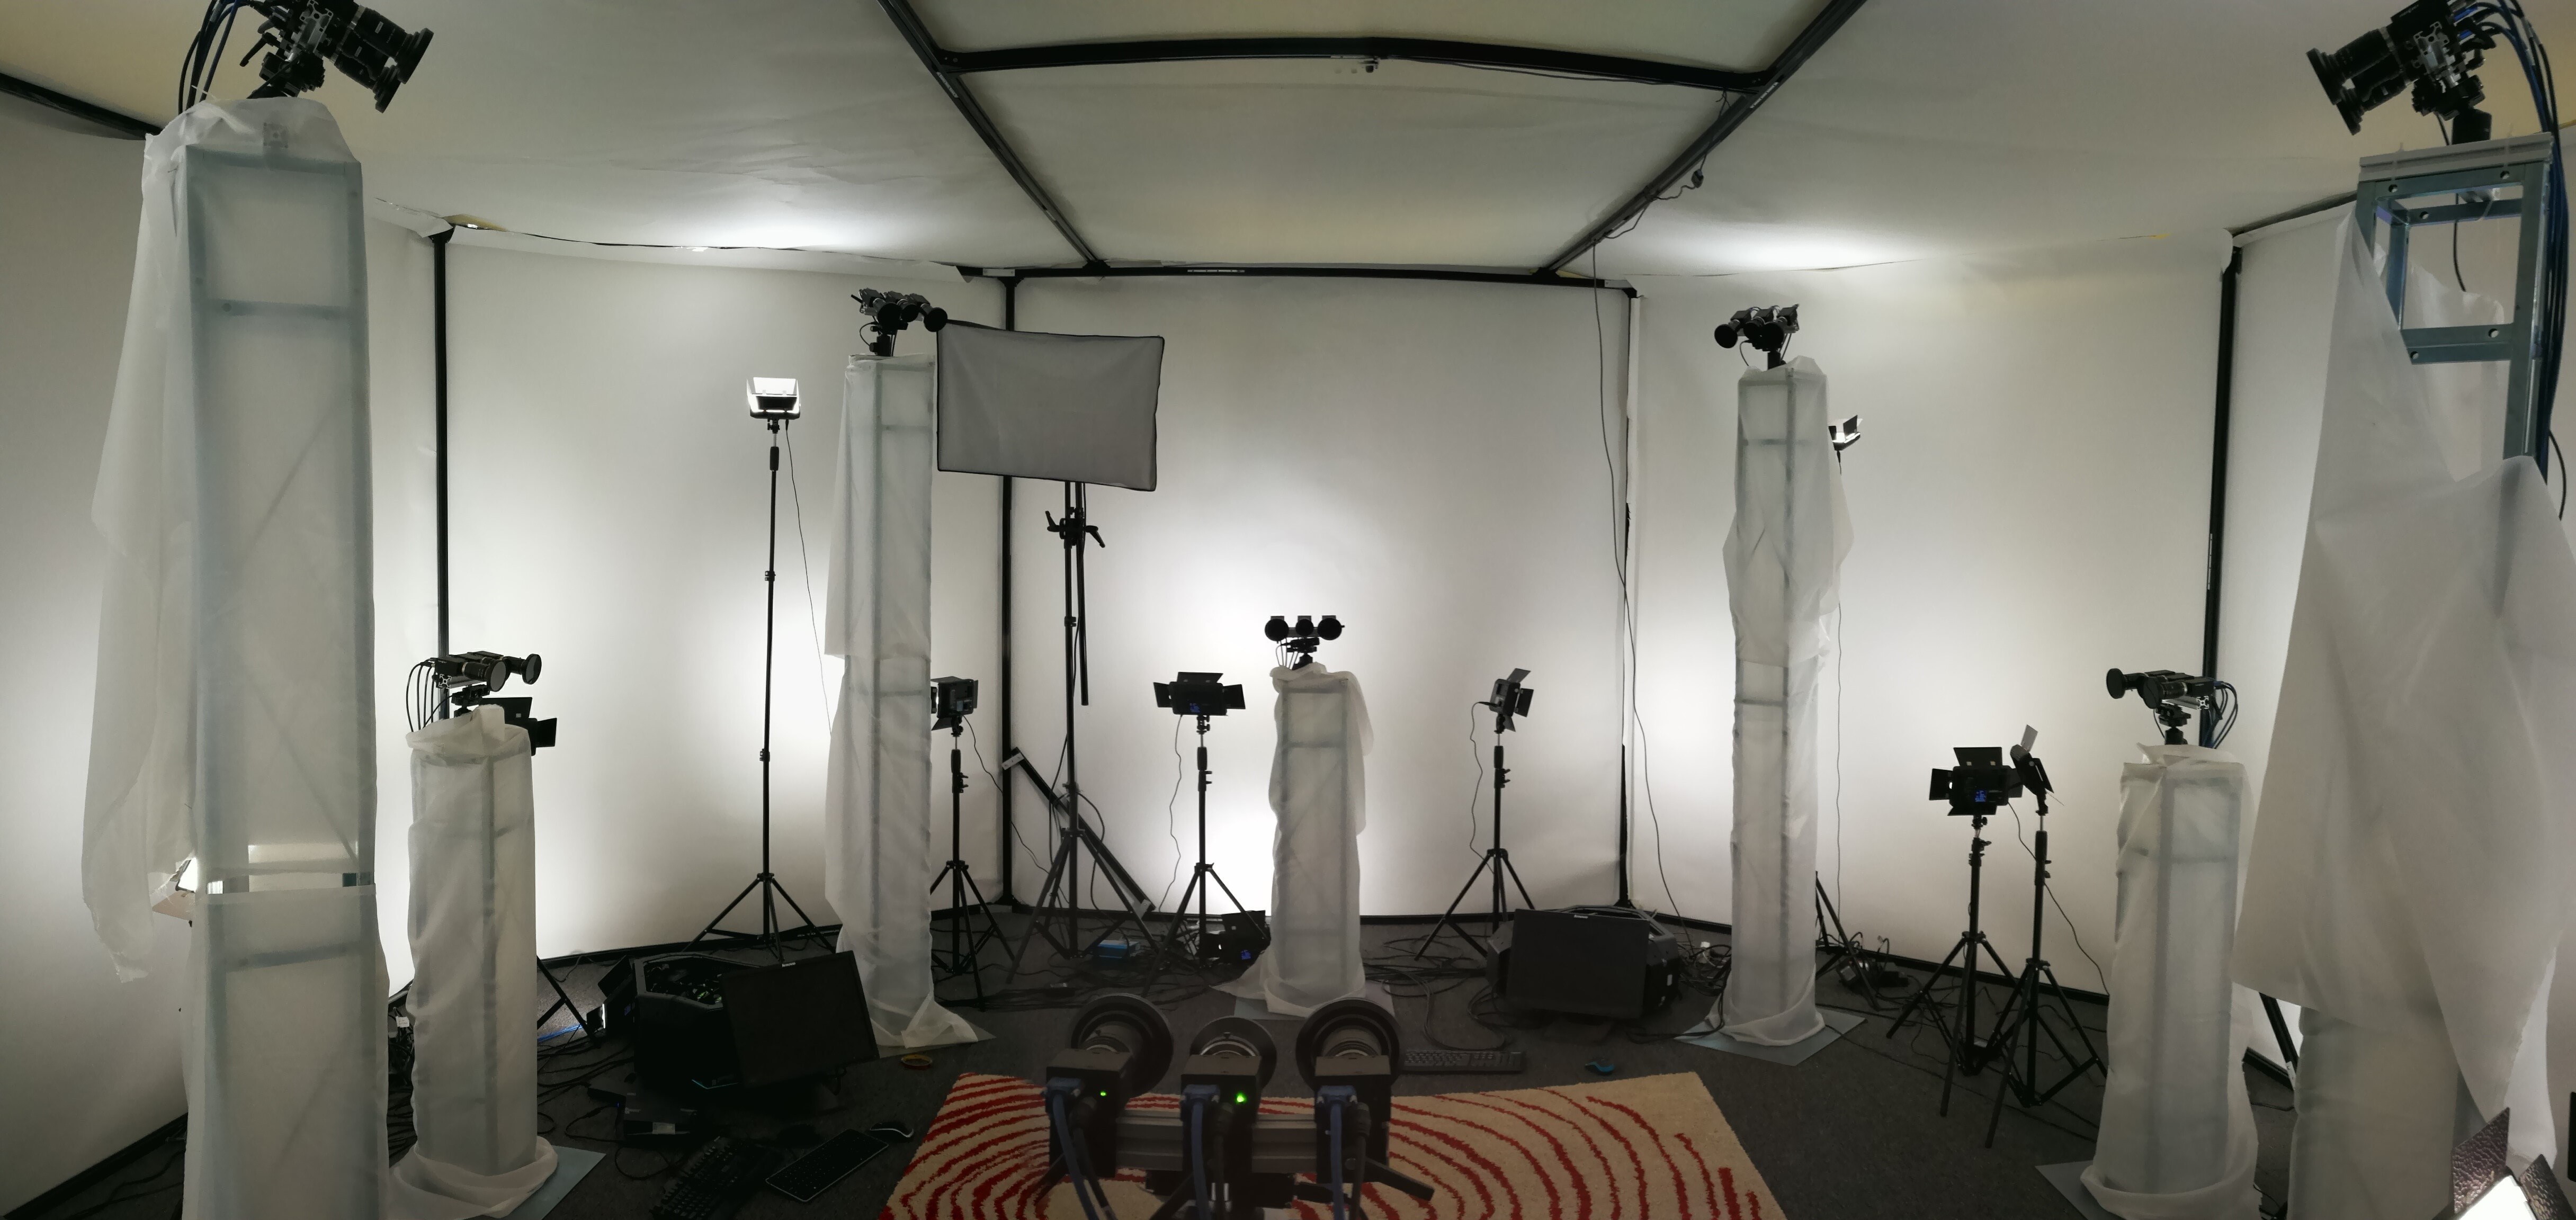
\includegraphics[scale=0.08]{image/rig.jpg}
\caption{Our multi-camera system with 8 camera pods pointing inwards.}
\label{fig:rig}
\end{figure*}

We employ 8 camera pods around the working space looking inwards for a full capture as shown in Figure~\ref{fig:rig}. Each camera pod consists of one color camera and two Near Infra-Red cameras. A laser pointer is used to produce special patterns.
From the two images of the projected patterns captured by the two NIR cameras, a depth map can be estimated using \xj{what algorithm?}
% it depth images can be achieved by the 2  using depth estimation methods.


%\subsection{Camera model}
Let $\mathbf{p}=(x,y,z,1)^{T}$ be the homogeneous coordinate of a point $P$ in the 3D space, and $\mathbf{x}=(u,v,1)^{T}$ the homogeneous coordinates of its projected point on an image plane, the perspective projection of a pin-hole camera is usually described as
\begin{equation}
z_{p}\mathbf{x}=\mathbf{K}\mathbf{M}\mathbf{p},
\end{equation}
where $z_{p}$ is the projective depth of point $P$, $\mathbf{K}$ and $\mathbf{M}$ are the intrinsic and extrinsic parameters of the camera.

%\subsection{Initial calibration}
The $\mathbf{K}$ and initial $\mathbf{M}$ of each camera are calibrated by Kalibr~\cite{Maye2013Self} pairwisely because of the lack of the common overlapping fields of view, including the 8 color cameras' extrinsic parameters $\{\mathbf{M}_{i}\}_{i=1,...,8}$. The extrinsic parameters from the 2 NIR cameras to the color camera in the same camera pod are also achieved, but these extrinsic parameters are fixed and used to estimate the depth in each view.

%\subsection{Global optimization}

We use a $6\times7$ checkerboard with squares of 117 mm for the optimization. 
\xj{Why do you need checkerboard? Why do you use 6x7 rather than other pattern?}
%
The user is requested to move the checkerboard in front of the cameras freely in the working space. The checkerboard can be simultaneously seen in three or four views usually. 
%
Then the 42 corners on the checkerboard can be detected in each group. 
%
We can estimate the 3D coordinates $\mathbf{P_{c}}$ of each corner from the corresponding 2D coordinates $\{\mathbf{p_{c}}_{j}\}_{j=1,...,n}$ by triangulation, where $n$ is the number of the views that the checkerboard can be seen in at the same time. 
To make the optimization result be more consistent to the whole system, we also use the images with checkerboard on the ground which allows the checkerboard corners can be seen in all the 8 cameras,  as shown in Figure~\ref{fig:checkerboard}. This will help to reduce the accumulative error and inconsistence caused by the pairwise calibration. 
The aim of the optimization is to minimize the sum of all reprojection errors with respect to all 3D points and extrinsic parameters, which is described as
\begin{equation}
E(\{\mathbf{K_{ex}}_{i}\})=\sum_{i}\sum_{j}((\mathbf{K_{in}}_{i}\mathbf{K_{ex}}_{i}\mathbf{P_{c}}_{j})-\mathbf{p_{c}}_{ij})^{2}.
\end{equation}
\xj{Do you only optimize the camera extrinsic parameters? How about the point coordinates?}
We use an open source software package called sba to solve this problem~\cite{lour09}.


\begin{figure}[ht]
%
\begin{minipage}[b]{.48\linewidth}
  \centering
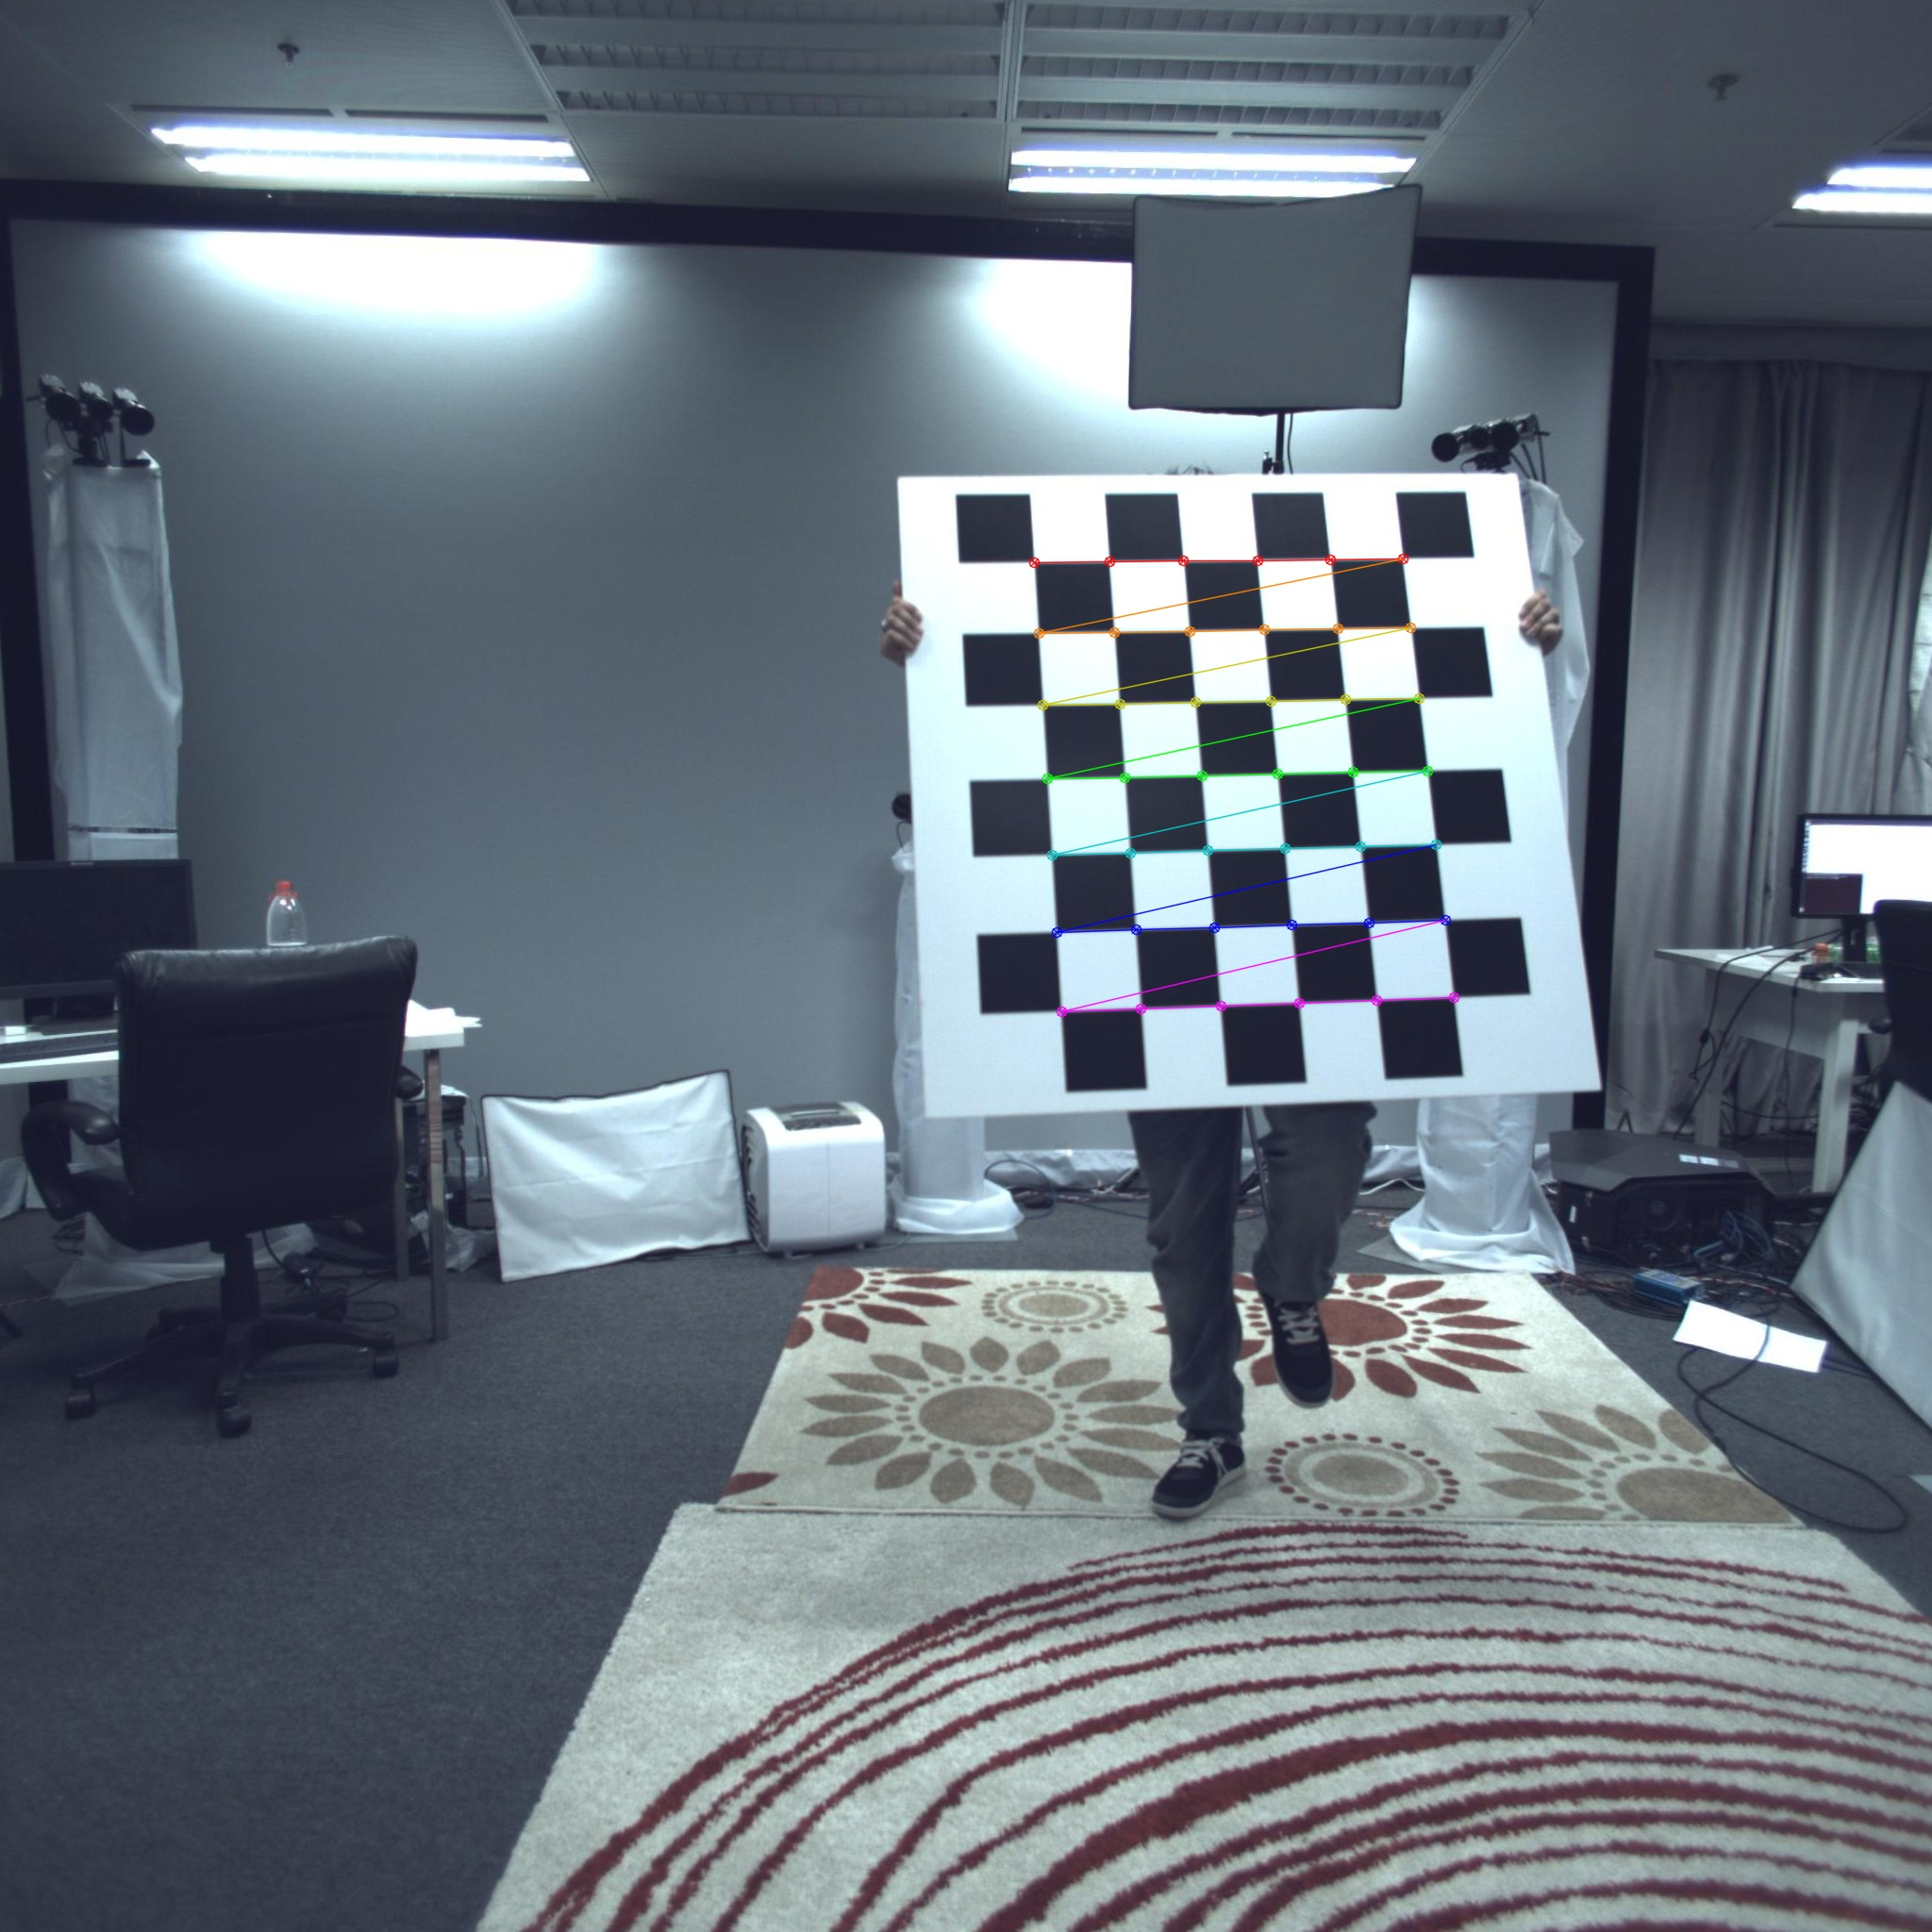
\includegraphics[scale=0.058]{image/free.jpg}
  \vspace{0cm}
  \centerline{(a)}\medskip
\end{minipage}
\hfill
\begin{minipage}[b]{0.48\linewidth}
  \centering
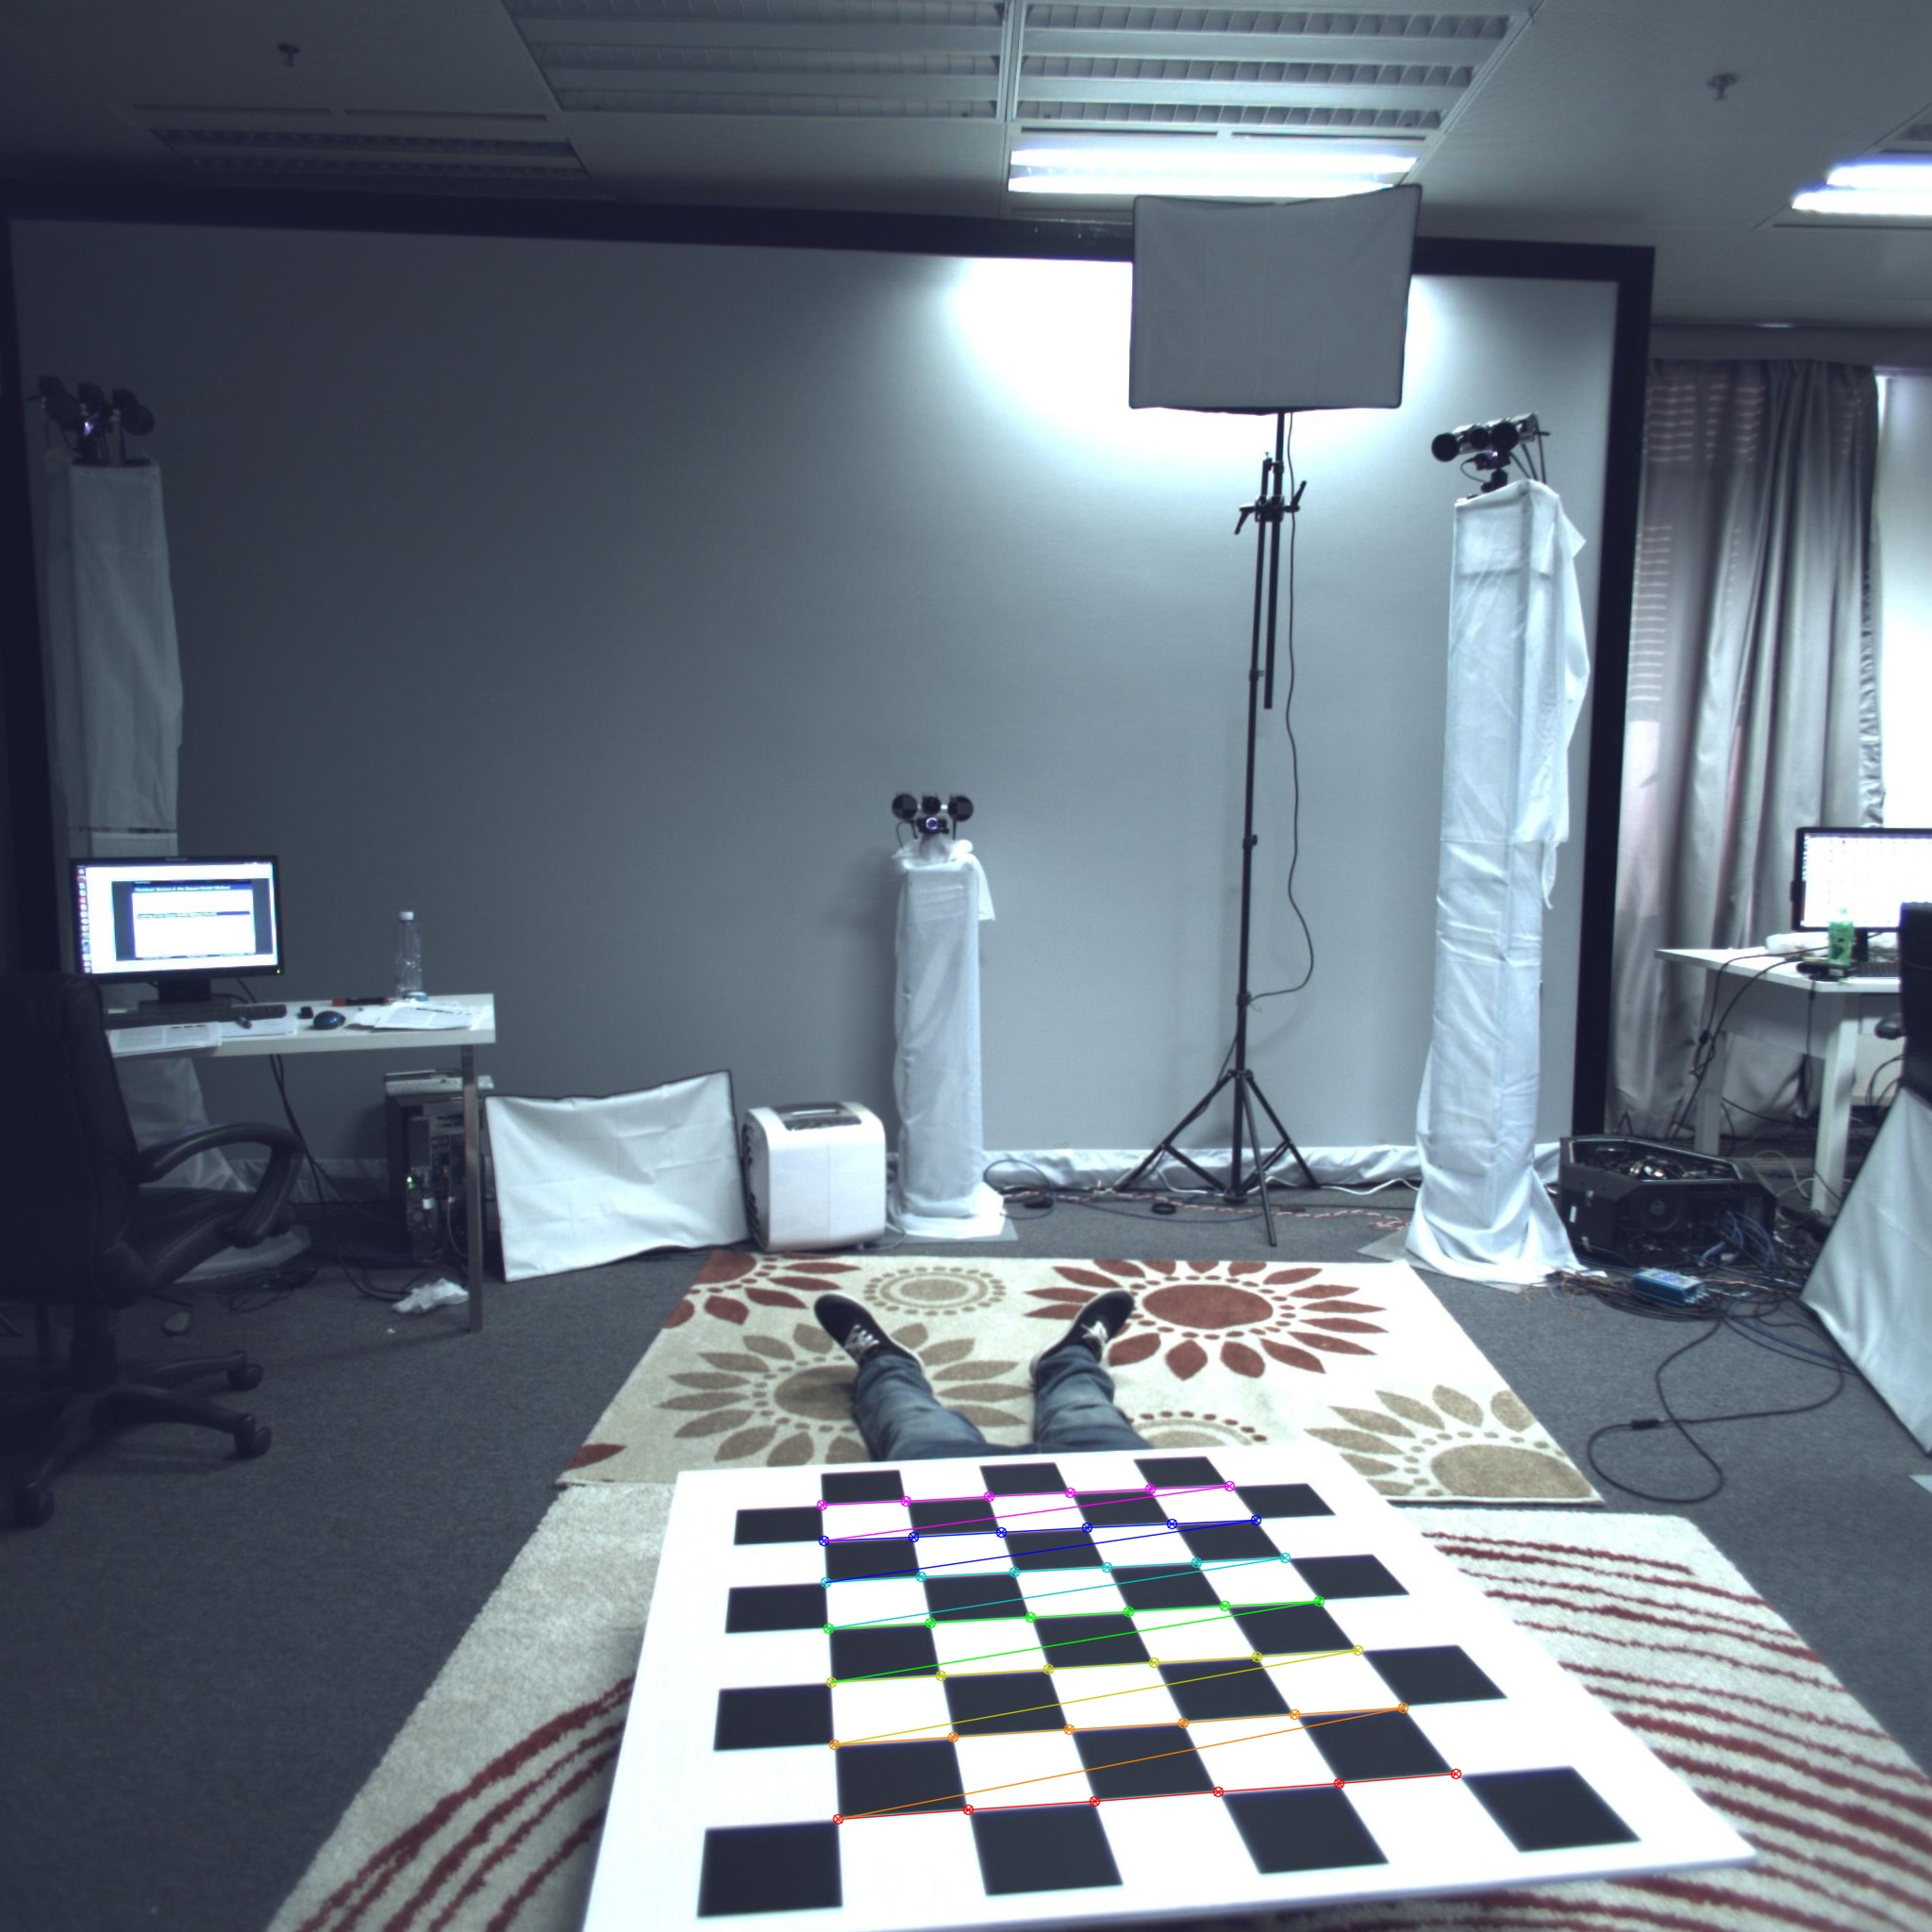
\includegraphics[scale=0.058]{image/ground.jpg}
  \vspace{0cm}
  \centerline{(b)}\medskip
\end{minipage}
%
\caption{Results of the checkerboard corners detection. (a): Results when the user moves freely. (b): Results when the checkerboard is on the ground. }
\label{fig:checkerboard}
\end{figure}



\section{point cloud registration}
\label{sec:registration}

We achieve the depth data from the 2 NIR cameras using depth estimation methods~\cite{Bleyer2011PatchMatch}. Although after the global optimization, we can get a result with less reprojection error, but it may not be the optimal solution to the 3D reconstruction because the quality of depth estimation also influence the final result. If the depth and camera parameters are both accurate enough, the point clouds of different views should align very well. 
However, the error cannot be avoided completely.
\xj{what error? caused by what?}

We reconstruct the point cloud of one view using the depth data, found the distortion on the boundary of the model, especially near the head, as shown in Figure~\ref{fig:deptherror}. Moreover, although the reprojection error after the global optimization mentioned in the last section is at sub-pixel level, we also find the separation between the point cloud of different views, effecting the quality of reconstruction. 
%
To minimize the error from depth data and achieve high-quality reconstruction results, we use ICP to map the inaccurate depth to a 3D model by point cloud registration.
\begin{figure}[ht]
\centering
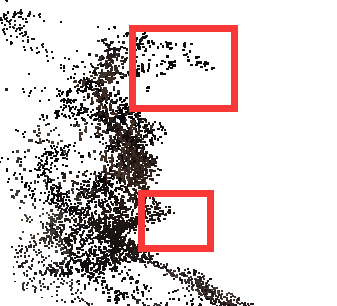
\includegraphics[scale=0.4]{image/depth_error.png}
\caption{The distortion near the head of the model of a single view which is caused by the inaccurate depth estimation. \xj{It is not clear. show a rgb image? or depth map from the camera view?}}
\label{fig:deptherror}
\end{figure}



For each point reconstructed by the depth image, we consider an estimation
\begin{equation}
\mathbf{\tilde{P}}_{ij}=f_{i}(\mathbf{P}_{j}),
\end{equation}
where $\mathbf{P}_{j}$ is the true 3D coordinates in the camera coordinate system. $f_{i}$ is a nonlinear function for view $i$, represent the depth influence. $\mathbf{\tilde{P}}_{ij}$ is the 3D coordinates we get from the depth data and intrinsic parameters in view $i$. With the extrinsic parameter, we can transform all the points into the world coordinate system. The estimation can be written as
\begin{equation}
\mathbf{\hat{P}}_{gj}=g(\mathbf{K_{ex}}_{i})f_{i}(\mathbf{P}_{j}),
\end{equation}
where $\mathbf{\hat{P}}_{gj}$ is the 3D coordinates in the world coordinate system we reconstruct from the depth and camera parameters. ICP can be replaced as a rigid transform to all views
\begin{equation}
\mathbf{\tilde{\hat{P}}}_{gj}=M_{i}g(\mathbf{K_{ex}}_{i})f_{i}(\mathbf{P}_{j})=g(\mathbf{K_{ex}}_{i})M_{i}f_{i}(\mathbf{P}_{j}),
\end{equation}
where $\mathbf{\tilde{\hat{P}}}_{gj}$ is the coordinates of the point after the alignment. The transform $M_{i}$ can refine the error caused by $f_{i}$, and improve the quality of the result of 3D reconstruction.

We choose the point cloud of view 1 as the reference, align the point cloud of view 2 to it, combine the result of the two views, then align the point cloud of view 3 to the combined result and so on. Each ICP process produce a transformation matrix, then we can map the inaccurate depth to a high-quality 3D model using the rigid transformation.


\xj{Show depth maps from 8 views. Show three fused models from pairwisely estimated camera parameters, globally estimated camera parameters, and after icp registration.  }


% References should be produced using the bibtex program from suitable
% BiBTeX files (here: strings, refs, manuals). The IEEEbib.bst bibliography
% style file from IEEE produces unsorted bibliography list.
% -------------------------------------------------------------------------
 